\documentclass[11pt]{article}
\usepackage[utf8]{inputenc}
\usepackage[T1]{fontenc}
\usepackage{amsmath, amssymb, amsfonts}
\usepackage{graphicx}
\usepackage{hyperref}
\usepackage{geometry}
\geometry{margin=1in}
\usepackage{float}
\usepackage{graphicx}
\usepackage{subcaption}

\title{Pricing European Call Options using Discrete Time Quantum Walks and Iterative Amplitude Estimation}
\author{
  Aaditeya Tripathi\thanks{California State University, East Bay} \and
  Anany Pravin\thanks{University of Illinois, Urbana-Champaign}
}
\date{\today}


\begin{document}
\maketitle

\begin{abstract}
We present a hybrid classical–quantum framework for pricing European call options by modeling asset dynamics using a discrete–time quantum walk (DTQW) over a log–price lattice and estimating expected payoffs via the Iterative Amplitude Estimation (IAE) algorithm  \cite{grinko2019iterative}. The underlying asset’s price evolution is encoded as a quantum superposition across discretized log–price states, where interference patterns capture non-Gaussian effects such as skew and fat tails. An exact amplitude oracle encodes the option payoff function, allowing IAE to estimate the expected payoff amplitude with quadratic speedup over classical Monte Carlo. We benchmark the quantum-derived prices against Black–Scholes valuations across various strike and volatility regimes using real market data (e.g., NVDA, AAPL), and observe consistent trends: close agreement in low-volatility regions and systematic quantum overpricing in tail-heavy or high-volatility environments. Statistical tests and 3D deviation surfaces confirm that these discrepancies reflect the model’s enhanced sensitivity to path structure. Our findings suggest that DTQW-based quantum pricing offers a controllable yet expressive alternative to classical diffusion-based models, and opens new avenues for capturing realistic market behaviors in near-term quantum finance.
\end{abstract}


\section{Introduction}

Accurate pricing of derivative securities lies at the heart of quantitative finance, where it informs trading strategies, hedging, and risk management. The Black--Scholes--Merton (BSM) model provides a celebrated closed-form solution for European options, assuming that the underlying asset follows a geometric Brownian motion with constant volatility \cite{black1973pricing}. However, real-world markets frequently violate these assumptions, exhibiting features such as volatility clustering, discontinuous price jumps, and heavy-tailed return distributions—features that challenge the fidelity of purely Gaussian models.

Quantum computing offers a new computational paradigm capable of addressing these limitations through principles like superposition and interference. In particular, amplitude-based algorithms such as \emph{Amplitude Estimation} (AE) provide a quadratic improvement over classical Monte Carlo methods in estimating expected values. This paper explores the application of near-term quantum algorithms to option pricing by simulating the underlying asset's dynamics using a discrete-time quantum walk (DTQW) over a log-price lattice. The option payoff is encoded exactly using Qiskit's \texttt{LinearAmplitudeFunction}, allowing us to avoid piecewise approximation. We then use Iterative Amplitude Estimation (IAE), a sampling-efficient variant of AE compatible with current hardware, to compute the expected discounted payoff under the risk-neutral measure. The resulting quantum price is benchmarked against the classical Black--Scholes price across varying strikes and volatilities, highlighting structural differences that emerge from the quantum walk’s non-Gaussian diffusion \cite{wang2022quantum}.

By replacing the continuous Brownian motion with a reversible unitary evolution, and integrating amplitude-based inference, this work builds a bridge between derivative finance and quantum computing. Our approach offers a natural way to encode fat tails, skewness, and path interference into asset dynamics, suggesting that quantum walks may serve as a compelling alternative foundation for option pricing in the post-classical era.


\section{Financial Preliminaries}
A European call option gives the holder the right but not the obligation to purchase the underlying
asset at a fixed price $K$ on a specific maturity date $T$. The terminal payoff
is:
\begin{equation}
\Pi(S_T) = \max(S_T - K, 0).
\end{equation}

Under the risk--neutral measure $\mathbb{Q}$, the price of the option is the
discounted expected value:
\begin{equation}
C = e^{-rT} \mathbb{E}_\mathbb{Q}[\Pi(S_T)\mid S_0].
\end{equation}

The Black--Scholes formula for a European call option with constant volatility
$\sigma$ is:
\begin{equation}
C_{BSM} = S_0 N(d_1) - K e^{-rT} N(d_2),
\end{equation}
where:
\begin{align}
d_1 &= \frac{\ln(S_0/K) + (r + 0.5\sigma^2)T}{\sigma \sqrt{T}}, \\
d_2 &= d_1 - \sigma \sqrt{T}.
\end{align}

\section{Quantum Computing Background}

Quantum computing generalizes classical computation by exploiting principles such as superposition, entanglement, and interference. The basic unit of quantum information is the \emph{qubit}, which is a normalized complex linear combination of two basis states:
\begin{equation}
|\psi\rangle = \alpha |0\rangle + \beta |1\rangle, \quad \text{with } \alpha, \beta \in \mathbb{C}, \quad |\alpha|^2 + |\beta|^2 = 1.
\end{equation}
Unlike classical bits, qubits can exist in a superposition of both $|0\rangle$ and $|1\rangle$ simultaneously, enabling massively parallel computations in certain algorithmic contexts.

A key primitive used in our model is the \textbf{discrete-time quantum walk} (DTQW), a quantum analog of classical random walks \cite{venegas2012quantum}. A DTQW consists of a \emph{coin qubit}, which determines the direction of movement, and multiple \emph{position qubits}, which encode the walker's location—in our case, mapped to a log-price lattice for asset dynamics. Each time step applies a coin rotation (typically a parameterized $R_y$ gate) followed by a conditional shift operation, where the coin state dictates the walker’s movement on the lattice. Repeating this sequence over several steps produces a probability amplitude distribution over asset prices, exhibiting quantum interference effects.

To extract expected payoffs from this distribution, we use \textbf{Iterative Amplitude Estimation} (IAE)—a near-term-compatible version of the Amplitude Estimation algorithm. IAE avoids the need for large-depth circuits by eliminating the use of controlled Grover powers, making it more suitable for noisy intermediate-scale quantum (NISQ) devices. It estimates the amplitude associated with a specific “good” state, which in our case corresponds to a normalized option payoff, achieving additive error $\varepsilon$ with only $\mathcal{O}(1/\varepsilon)$ calls \cite{grinko2019iterative} to the quantum circuit.

Together, the quantum walk and IAE form a hybrid algorithm: the walk evolves a superposition over asset prices, and IAE infers the expected discounted payoff encoded as an amplitude, which we then scale to obtain the final option price. This combination allows us to represent non-Gaussian behavior and perform probabilistic inference with a potential speed advantage over classical Monte Carlo methods.


\section{Quantum Option Pricing Model}

In our framework, the underlying asset price is modeled as a discrete--time quantum walk (DTQW) evolving on a one--dimensional log--price lattice. This approach provides a quantum analog to the classical geometric Brownian motion used in the Black--Scholes model.

\subsection{Log--Price Encoding and Quantum Walk}

We encode the asset's log--price as a position state on a lattice of $2^n$ nodes, where $n$ is the number of position qubits. Let $x \in \{-N, \ldots, N\}$ represent the displacement from the initial log--price. The corresponding asset price at each node is:
\begin{equation}
S(x) = S_0 \exp(x \cdot \delta),
\end{equation}
where $\delta = \sigma \sqrt{T / M}$ is the log--price increment, $\sigma$ is the annualized volatility, $T$ is the time to maturity, and $M$ is the number of time steps in the walk.

A single step of the DTQW applies:
\begin{enumerate}
\item a coin rotation $R_y(\theta)$ to a control qubit, and
\item a position shift conditional on the coin state, implementing interference patterns in the log--price space.
\end{enumerate}

The rotation angle $\theta$ is derived from the drift-adjusted risk--neutral probability:
\begin{equation}
p = \frac{1}{1 + \exp(-2\mu_{\mathbb{Q}}/\sigma^2)}, \quad \theta = 2 \arcsin(\sqrt{p}),
\end{equation}
where $\mu_{\mathbb{Q}} = r - \frac{1}{2}\sigma^2$ is the risk-neutral drift.

\subsection{Expected Payoff as Amplitude}

After $M$ quantum walk steps, the final state is a superposition of all reachable log--prices:
\begin{equation}
|\psi_T\rangle = \sum_x \alpha_x |x\rangle,
\end{equation}
where $|\alpha_x|^2$ gives the probability of ending at node $x$ (log-price $S(x)$). The call option payoff is evaluated pointwise as $\Pi(x) = \max(S(x) - K, 0)$.

To compute the expected payoff, we construct a quantum amplitude function $f(x)$ normalized to $[0,1]$, such that:
\begin{equation}
f(x) = \frac{\Pi(x)}{\max_x \Pi(x)}.
\end{equation}

This function is encoded using a `LinearAmplitudeFunction` and applied as an oracle to the quantum state. We then apply Iterative Amplitude Estimation (IAE) to estimate the amplitude:
\begin{equation}
\mathbb{E}_\mathbb{Q}[\Pi(S_T)] \approx \hat{a} \cdot \max_x \Pi(x),
\end{equation}
and discount it using $e^{-rT}$ to obtain the quantum option price,
\begin{equation}
C_{\text{quantum}} = e^{-rT} \cdot \max_x \Pi(x) \cdot \hat{a}
\end{equation}


\subsection{Summary}

This model replaces the continuous diffusion of classical models with a discrete quantum walk, while preserving the probabilistic interpretation of final prices. The use of quantum amplitudes allows us to encode richer path interference effects, enabling the study of non-Gaussian features such as fat tails and volatility clustering.



\section{Methodology}
We construct a quantum circuit comprising:
\begin{itemize}
\item a quantum walk on log--price space,
\item an exact payoff oracle mapping grid points to amplitudes, and
\item IAE to extract the amplitude encoding expected payoff.
\end{itemize}

The payoff is scaled to $[0,1]$ using the maximum observed value to normalize the
amplitude function.

\section{Modeling Real Assets with Quantum Walks}
\label{sec:modeling_assets}

To investigate the practical behavior of our quantum pricing framework, we applied it to real market data for large-cap U.S. equities (data from Yahoo Finance using the yfinance API \cite{yfinance}), using Nvidia (NVDA) and Apple (AAPL) as representative examples of high- and low-volatility assets, respectively. We simulated European call options and compared quantum-derived prices with the classical Black--Scholes--Merton (BSM) values under varying market conditions.

\subsection{Strike-Dependent Quantum Pricing Across Assets}

We first examined how quantum option prices respond to moneyness by simulating call prices over a range of strike values $K \in [0.8S_0, 1.2S_0]$ for a fixed maturity of $T = 250$ days. Figures~\ref{fig:quantum_strike_sweep_nvda} and \ref{fig:quantum_strike_sweep_aapl} illustrate pricing curves for NVDA and AAPL, respectively.

In both cases, quantum prices decrease monotonically with strike, consistent with financial intuition. However, the magnitude of divergence from BSM differs markedly by asset. For NVDA, which has historically higher volatility, quantum prices remain elevated across strikes, indicating that the quantum walk disproportionately assigns amplitude to high-payoff paths. For AAPL, a lower-volatility stock, quantum and classical prices align more closely.

These results suggest that quantum walks naturally express fat-tailed distributions and asymmetry in price outcomes, offering an alternate way to incorporate skew and kurtosis without modifying the payoff structure or volatility surface.

\begin{figure}[H]
    \centering
    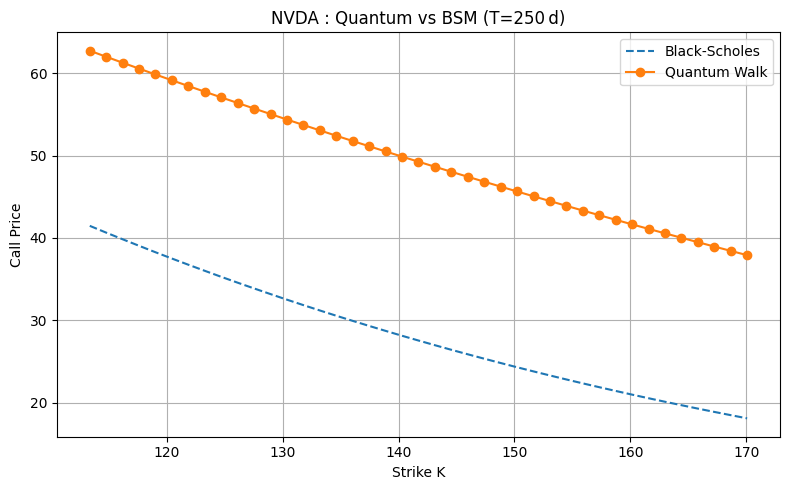
\includegraphics[width=0.75\textwidth]{QvBSM_K(img).png}
    \caption{Quantum vs Black--Scholes call prices across strike prices for NVDA ($T = 250$ days). The quantum model shows consistent overpricing relative to Black--Scholes.}
    \label{fig:quantum_strike_sweep_nvda}
\end{figure}

\begin{figure}[H]
    \centering
    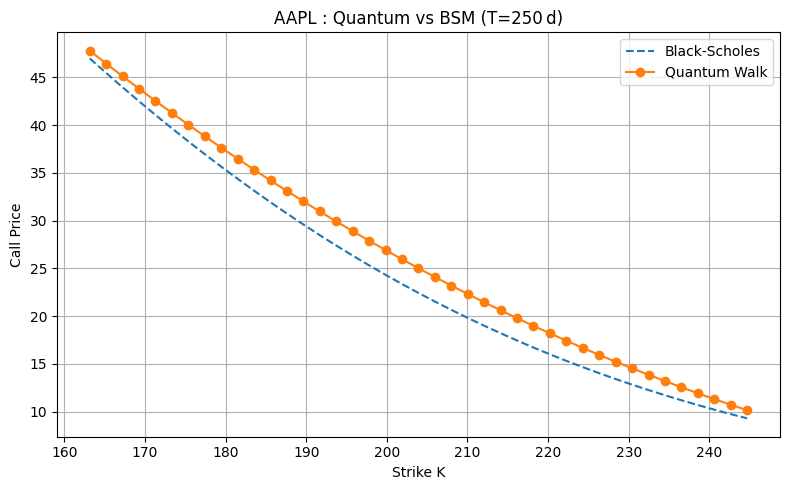
\includegraphics[width=0.75\textwidth]{QvBSM_K_AAPL(img).png}
    \caption{Quantum vs Black--Scholes call prices across strike prices for AAPL ($T = 250$ days). Quantum and classical prices remain close, with minor elevation in quantum estimates.}
    \label{fig:quantum_strike_sweep_aapl}
\end{figure}

\subsection{Volatility Amplification and Controlled Quantum Pricing}

We next explored how option prices vary with volatility. Figure~\ref{fig:quantum_volatility_comparison} shows simulated prices across a range of annualized volatilities $\sigma \in [0.1, 1.2]$, using $K = 1.05 \cdot S_0$ and $T = 250$ days.

In the uncontrolled case (left panel), prices increase rapidly with volatility, reaching values exceeding \$500. This "volatility blow-up" results from the broad dispersion of the quantum walk, which increases the range of reachable payoffs and feeds directly into the amplitude oracle.

To counteract this, we introduce a constraint by setting $\texttt{span\_sigma} = 2$, which narrows the effective diffusion band. As shown in the right panel, this controlled simulation tempers amplification while preserving sensitivity to volatility. The ability to tune this behavior makes the model adaptable to different risk profiles and use cases.

\begin{figure}[H]
    \centering
    \begin{subfigure}[b]{0.48\textwidth}
        \centering
        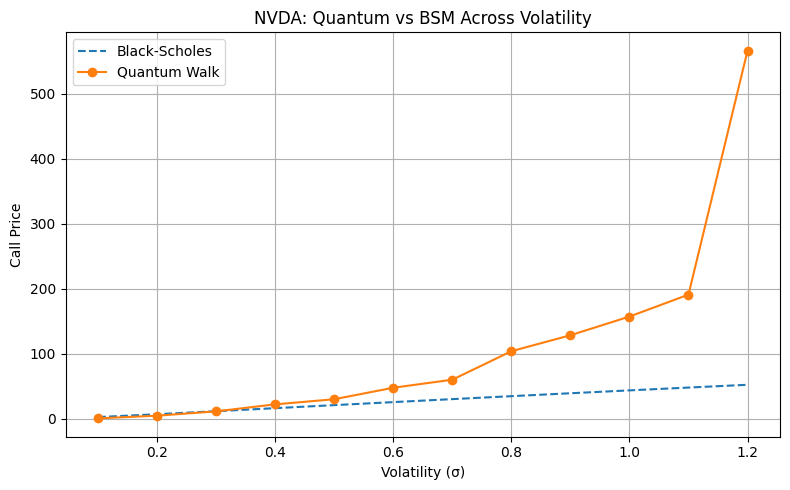
\includegraphics[width=\linewidth]{QvBSM_Uncontrolled(img).png}
        \caption{Uncontrolled ($\texttt{span\_sigma} = 3$)}
        \label{fig:quantum_uncontrolled}
    \end{subfigure}
    \hfill
    \begin{subfigure}[b]{0.48\textwidth}
        \centering
        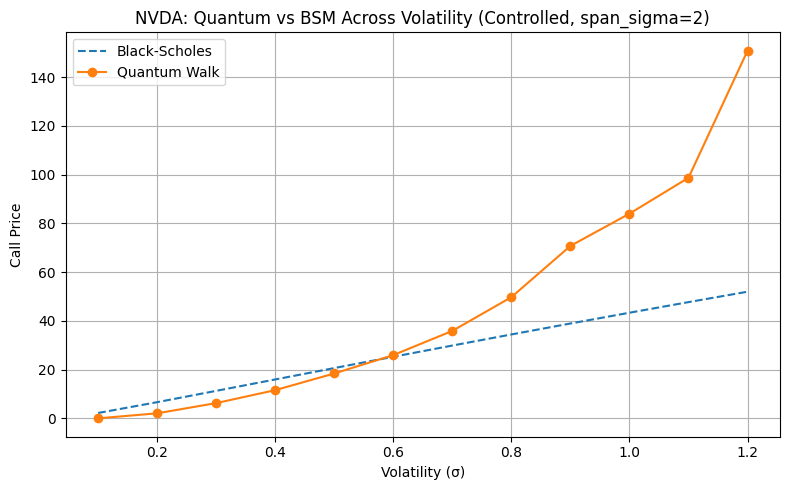
\includegraphics[width=\linewidth]{QvBSM_Controlled(img).png}
        \caption{Controlled ($\texttt{span\_sigma} = 2$)}
        \label{fig:quantum_controlled}
    \end{subfigure}
    \caption{Quantum vs Black--Scholes call prices across volatility. The quantum model shows increasing divergence from classical pricing as volatility rises. Controlled spread (b) avoids pathological blow-up while retaining high sensitivity.}
    \label{fig:quantum_volatility_comparison}
\end{figure}

\subsection{Volatility-Maturity Surface Visualization}

We visualized QOP-BSM price deviations over a grid of volatilities ($\sigma \in [0.1, 1.2]$) and maturities ($T \in [0.1, 5.0]$) using a 3D surface plot. The surface clearly delineates two behavioral zones:

\begin{itemize}
\item \textbf{Stable Zone (blue basin):} At low-to-moderate volatility and short-to-medium maturity, QOP pricing closely tracks BSM. 
\item \textbf{Explosive Zone (red ridge):} At high volatility and long maturity, QOP exhibits pronounced overpricing. This is consistent with quantum walk amplitude tails dominating payoff weights.
\end{itemize}

\begin{figure}[H]
\centering
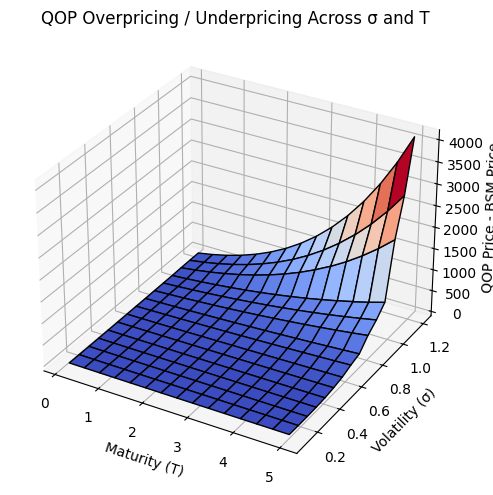
\includegraphics[width=0.75\textwidth]{QOPvsBSM_3Dplot.png}
\caption{Deviation surface showing $\text{QOP Price} - \text{BSM Price}$ over volatility $\sigma$ and maturity $T$. The red ridge indicates regions of significant overpricing in the quantum model.}
\label{fig\:qop\_bsm\_surface}
\end{figure}

\section{Are Deviations Features, Not Bugs?}

The Quantum Option Pricing (QOP) model exhibits systematic deviations from Black--Scholes--Merton (BSM) pricing in certain parameter regimes. These differences are not numerical artifacts or implementation errors, but rather emergent features rooted in the physics of quantum walk evolution and amplitude-based expectation estimation.

Classical models assume log-normal returns driven by Gaussian diffusion, which strongly dampens the probability of large deviations from the mean. In contrast, quantum walks distribute amplitude over log-price trajectories using interference. Constructive interference can reinforce low-probability but high-payoff paths \cite{meyer1996quantum}, while destructive interference can suppress paths that contribute minimally to the payoff. This mechanism enables QOP to organically encode fat tails, skew, and asymmetric return structures.

Moreover, the Iterative Amplitude Estimation (IAE) algorithm used to extract expected payoffs does not impose linear scaling with variance. As volatility increases, the distribution of amplitudes becomes more dispersed, and the contribution of high-payoff nodes can be magnified—particularly if no bounding mechanism (like $\texttt{span\_sigma}$) is imposed. These effects may appear as "overpricing" when judged against BSM, but in fact reflect the richer expressive capacity of QOP.

\begin{quote}
\textit{What might initially appear as a pricing anomaly is, in truth, a deliberate byproduct of the quantum framework’s ability to capture nonlinear price dynamics and tail-driven behavior.}
\end{quote}

This characteristic is not a defect but an advantage in markets where BSM assumptions fail—for instance, during earnings shocks, financial crises, or periods of elevated implied volatility.

\vspace{0.3cm}

\subsection{Inference}

Our results confirm that the QOP model behaves reliably and in close agreement with classical benchmarks under standard market conditions—specifically, when volatility is moderate ($\sigma \lesssim 0.4$) and the time to maturity is short ($T \lesssim 0.5$ years). In these domains, quantum prices exhibit only mild deviation from BSM values and remain interpretable.

However, in high-volatility or long-dated scenarios, quantum prices begin to diverge significantly. This divergence is not uniform, but parameter-sensitive: it intensifies when both volatility and maturity are high, particularly in out-of-the-money regions where classical models assign negligible value. These cases are precisely where classical diffusion-based models tend to underestimate optionality \cite{baaquie2007quantum}.

\begin{quote}
\textit{Thus, while QOP provides a robust and expressive framework for option pricing, its application must be guided by an understanding of when quantum effects—such as amplitude amplification and interference—become dominant.}
\end{quote}

In summary, the QOP model is not merely a quantum reinterpretation of BSM—it is a distinct pricing paradigm capable of representing richer market dynamics, provided its use is informed by careful analysis of its strengths and sensitivities.


\section{Limitations}

While our quantum walk–based option pricing framework provides new modeling capabilities and demonstrates promising results, several limitations must be acknowledged:

\begin{itemize}
    \item \textbf{Noisy Intermediate-Scale Quantum (NISQ) Constraints}: All simulations were conducted on classical simulators. Current quantum hardware suffers from limited qubit fidelity, decoherence, and gate noise, which can significantly impair the accuracy of amplitude estimation.
    
    \item \textbf{Lattice Granularity and Discretization Bias}: The log–price lattice used in the discrete–time quantum walk introduces discretization artifacts. Finer lattices improve accuracy but require more qubits and deeper circuits, which are currently resource-intensive.
    
    \item \textbf{Path-Independent Payoff Limitation}: The model is designed for European-style options with terminal payoffs. Extending the framework to handle path-dependent options (e.g., Asian or barrier options) would require more sophisticated oracle constructions and larger circuits \cite{schuld2015introduction}.
    
    \item \textbf{Parameter Sensitivity}: The quantum price is highly sensitive to volatility $\sigma$ and the span control parameter \texttt{span\_sigma}. Poor calibration can lead to unrealistically amplified prices or instability under high volatility and long maturity.
    
    \item \textbf{Scalability Constraints}: The use of 4–5 qubits limits the number of resolvable price states on the lattice. Increasing resolution necessitates additional qubits, posing scalability and performance challenges.
    
    \item \textbf{Absence of Closed-Form Analytical Bounds}: Unlike the Black–Scholes model, the quantum pricing method lacks closed-form expressions for key sensitivities like delta or gamma, making financial interpretation and risk management less direct.
\end{itemize}

These limitations define the current boundary of the model’s applicability while highlighting avenues for future research in quantum finance.



\section{Conclusion}
We developed a quantum-inspired framework for pricing European call options by modeling asset dynamics as a discrete--time quantum walk and applying Iterative Amplitude Estimation to extract expected payoffs. Our method captures interference patterns over a log--price lattice, offering a quantum analog to the geometric Brownian motion in Black--Scholes. Numerical results across real market data show that the quantum prices remain consistent with classical benchmarks in low-volatility settings, while demonstrating amplified sensitivity under higher volatility and strike variations.

This framework showcases how quantum walks can encode richer structural properties—such as heavy tails and nonlinear dispersion—without abandoning financial interpretability. The model is fully programmable using Qiskit, and deployable for testing on classical simulators or future quantum hardware.

Future work could extend this approach to barrier options, path-dependent payoffs, and stochastic volatility models, potentially leveraging adaptive coin operations or circuit-level noise calibration. As quantum processors mature, this line of research paves the way for practical quantum advantage in derivative pricing.


\bibliographystyle{plain}
\bibliography{refs}

\end{document}
